\ifx\PREAMBLE\undefined
\documentclass[fleqn]{article}
\usepackage{geometry}
\usepackage[format = hang, font = bf]{caption}
\usepackage{subcaption}
% The following is needed in order to make the code compatible
% with both latex/dvips and pdflatex. Added for using UML generated by MetaUML.
\ifx\pdftexversion\undefined
\usepackage[dvips]{graphicx}
\else
\usepackage[pdftex]{graphicx}
\DeclareGraphicsRule{*}{mps}{*}{}
\fi
\usepackage{array}
\newcolumntype{C}[1]{>{\centering\let\newline\\\arraybackslash}b{#1}}
\newcommand{\parcell}[2][l]{\begin{tabular}{@{}#1@{}}#2\end{tabular}}
\usepackage{pdflscape}
\usepackage{multirow}
\usepackage{graphicx}
\usepackage{floatrow}
\floatsetup[table]{capposition=top}
\usepackage{bigstrut}
\usepackage{supertabular}
\usepackage{booktabs}
\usepackage{amsmath}
\usepackage{listings}
\usepackage{multicol}
\usepackage{xcolor}
\usepackage{mathrsfs}%mathcal
\usepackage{amsfonts}%allowing \mathbb{R}
\usepackage{amssymb}
\usepackage{alltt}
\usepackage{xspace}
\usepackage{color}
\usepackage{wrapfig}%text around figure
\usepackage{lipsum}
\usepackage{tikz}
\usetikzlibrary{shapes,positioning}
\usepackage{url}
\def\UrlBreaks{\do\A\do\B\do\C\do\D\do\E\do\F\do\G\do\H\do\I\do\J\do\K\do\L\do\M\do\N\do\O\do\P\do\Q\do\R\do\S\do\T\do\U\do\V\do\W\do\X\do\Y\do\Z\do\[\do\\\do\]\do\^\do\_\do\`\do\a\do\b\do\c\do\d\do\e\do\f\do\g\do\h\do\i\do\j\do\k\do\l\do\m\do\n\do\o\do\p\do\q\do\r\do\s\do\t\do\u\do\v\do\w\do\x\do\y\do\z\do\0\do\1\do\2\do\3\do\4\do\5\do\6\do\7\do\8\do\9\do\.\do\@\do\\\do\/\do\!\do\_\do\|\do\;\do\>\do\]\do\)\do\,\do\?\do\'\do+\do\=\do\#\do\-}
\usepackage{xr}%allow cross-file references
\usepackage[breaklinks = true]{hyperref}
\lstset{
language = C, 
showspaces = false,
breaklines = true, 
tabsize = 2, 
extendedchars = false, 
basicstyle = {\ttfamily \footnotesize}, 
showstringspaces=false,
keywordstyle=\color{blue!70}, 
commentstyle=\color{gray},
rulesepcolor=\color{red!20!green!20!blue!20}, 
numberstyle=\color[RGB]{0,192,192},
stringstyle=\color{red},
escapeinside={ )},
moredelim=[is][\underbar]{(**}{**)},
mathescape
}
\mathchardef\myhyphen="2D
\begin{document}
\fi
\newpage
\section{Exception Control Flow}
Understanding ECF can help us
\begin{itemize}
\item Understand important concepts: IO, process, virtual memory, etc.
\item Understand how applications interact with the OS: writing data to disk, reading data from network, creating / terminating a process all involve a form of ECF known as \textbf{system call (trap)}.
\item Write interesting new programs such as Unix shells and web servers, using ECF mechanisms provided by the OS.
\item Understand concurrency.
\item Understand how software exceptions work in C++, JAVA, etc.
\end{itemize}
\subsection{Exception}
\subsubsection{Definition}
\begin{description}
\item[Exception]An abrupt change in the control flow in response to some change the processor's state. 
\item[Event]Change in a processor's state (encoded in various bits and signals). 
\begin{itemize}
\item Can be related to the execution of the current instruction: virtual memory page fault, arithmetic overflow, division by 0, etc.
\item Or unrelated: system timer goes off, I/O request completion.
\end{itemize}
When the processor detects an event, it makes an indirect procedure call (the exception), through a jump table called the \textbf{exception table}, to an OS subroutine (the exception handler). When the exception handler finishes processing, it either returns control to the current instruction or the next instruction, or aborts the program.
\item[Exception number]An unsigned integer assigned to each type of exception. 
\begin{itemize}
	\item By processor designer: division by 0, page fault, illegal memory access, break point, arithmetic overflow.
	\item By OS kernel designer: system call, signals from external IO devices.
\end{itemize}
\item[Exception table]Allocated at system boot time. Entry \emph{k} contains the address of the handler of exception \emph{k}. Its starting address is stored in a special CPU register called the \textbf{exception table base register}.
\end{description}
Exception is akin to procedure call except for some important differences:
\begin{itemize}
\item As with procedure call, the return address is pushed on the stack. But the return address can be the current or the next instruction.
\item The processor also pushes some additional processor state on the stack that will be necessary when the handler returns and the interrupted program continues, e.g. EFLAGS.
\item When control is transferred to the kernel, these items are pushed onto the kernel stack instead of the user stack.
\item Exception handlers run in kernel mode, thus have complete access to all system resources.
\end{itemize}
\subsubsection{Classes}
\begin{description}
	\item[Async]Not caused by any instruction.
	\item[Sync]Caused by the current instruction (the faulting instruction). 
\end{description}
\begin{table}[h]
\centering
\caption{Classes of exceptions}
\begin{tabular}{clcl}\toprule
Class & Cause & Async/Sync & Return address\\\midrule
Interrupt & Signal from IO devices & Async & The next instruction \\
Trap & Intentional exception & Sync & The next instruction\\
Fault & Potentially recoverable error & Sync & The current instruction\\
Abort & Non-recoverable error & Sync & Never returns\\\bottomrule
\end{tabular}
\end{table}
\begin{table}[h]
\centering
\caption{Example of x86-64 exceptions}
\begin{tabular}{c|l|c|l}\toprule
Number & Description & Class & Outcome\\\midrule
0 & \parcell{Division by 0\\ (Floating exception)}& Fault & No attempt to recover\\\midrule
13 & \parcell{General protection fault\\ (Segmentation fault)} & Fault & No attempt to recover\\\midrule
14 & Page fault & Fault & Maps disk page to memory page. \\\midrule
18 & \parcell{Machine check\\ (Fatal hardware error)} & Abort & \\\midrule
32-255 & OS defined exceptions & \parcell{Interrupt\\or trap} & \\\bottomrule 
\end{tabular}
\end{table}
\begin{description}
	\item[syscall]C function \& x86-64 instruction to make system calls. For the instruction:
	\begin{itemize}
		\item System call number: \texttt{\%rax}
		\item Arguments: \texttt{\%rdi, \%rsi, \%rdx, \%r10, \%r8, \%r9}
		\item Return value: \texttt{\%rax}. -4095 $\sim$ -1 indicates error, corresponding to negative \texttt{errno}.
		\item Registers destroyed: \texttt{\%rcx, \%r11}
	\end{itemize} 
\end{description}
``Hello world'' written using system-level function:
\begin{lstlisting}
int main() {
	write(1, "Hello, world\n", 13); //1: stdout. 13: number of bytes to write.
	_exit(0);
}
\end{lstlisting}
\begin{table}[ht]
\centering
\caption{Example of x86-64 system calls}
\begin{tabular}{c|>{\tt}c|l||c|>{\tt}c|l}\toprule
N.O.& \multicolumn{1}{c|}{Name} & Description & N.O. & \multicolumn{1}{c|}{Name} & Description \\\midrule
0 & read & Read file & 33 & pause & Suspend process until signal arrives\\
1 & write & Write file & 37 & alarm & Schedule delivery of alarm signal \\
2 & open & Open file & 39 & getpid & Get process ID\\
3 & close & Close file & 57 & fork & Create process\\
4 & stat & Get info about file & 59 & execve & Execute a program\\
9 & mmap & Map memory page to file & 60 & \_exit & Terminate process\\
12 & brk & Reset the top of the heap & 61 & wait4 & Wait for a process to terminate \\
32 & dup2 & Copy file descriptor & 62 & kill & Send signal to a process\\\bottomrule
\end{tabular}
\end{table}
\subsection{Processes}
\begin{description}
	\item[Process]An instance of a program in execution. Each program runs in the context of a process. A process provides to applications 2 key abstractions:
	\begin{itemize}
		\item An independent \textbf{logical control flow} that provides the illusion that this program has exclusive use of the processor.
		\item A \textbf{private address space} that provides the illusion that this program has exclusive use of the memory system. 
	\end{itemize}
	\item[Context]The state that the program needs to run correctly, including the program's code and data stored in the memory, its stack, general registers' contents, PC, environment variables, and the set of open file descriptors.
	\item[Concurrent flow]A logical flow whose execution overlaps with another logical flow. 
	\begin{description}
		\item[Concurrency]The general phenomenon of multiple flows executing concurrently.
		\item[Multi-tasking(time slicing)]The notion of a process taking turns with other processes. Processes get \textbf{preempted} by each other.
		\item[Time slice]Each time period that a process executes a portion of its flow.
		\item[Parallel flows]A proper subset of concurrent flows: two flows running concurrently on different processor cores or computers.
	\end{description}
	\item[Private address space]Private in the sense that the byte related to an address cannot be read/written by other processes. 
	\begin{figure}[ht]
	\centering
	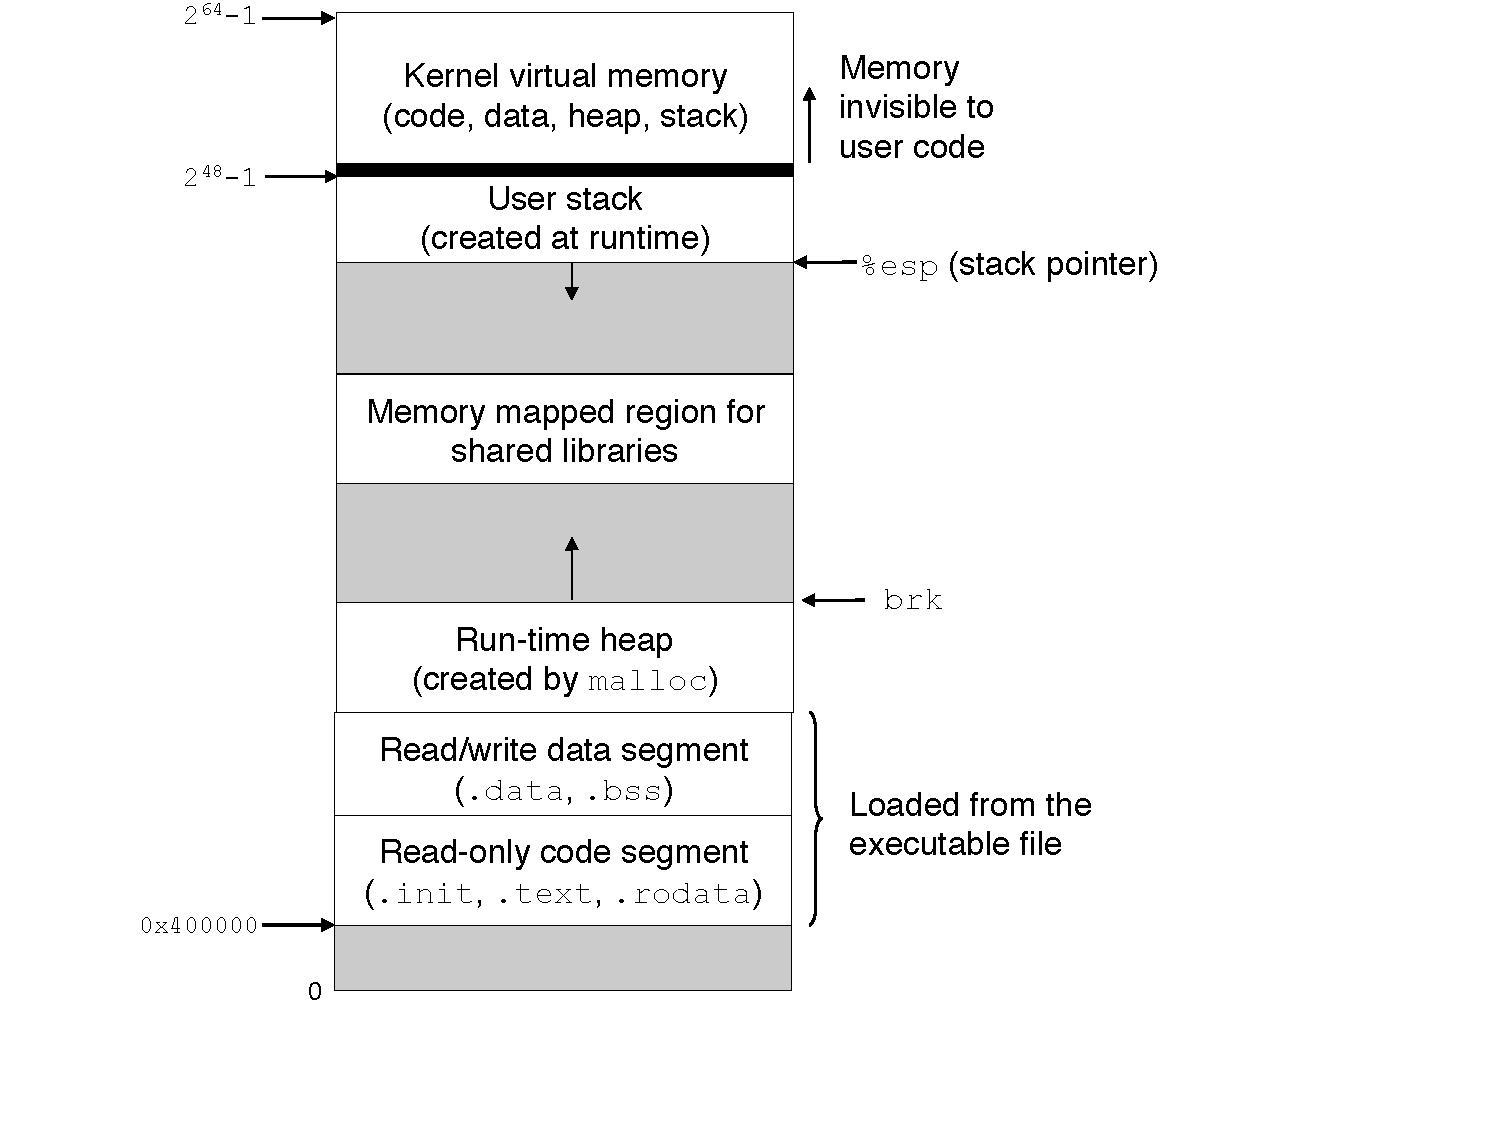
\includegraphics[width=0.5\textwidth]{addrspace.pdf}
	\caption{Structure of private address space}
	\end{figure}
	\item[User/Kernel mode] A mechanism provided by the processor to restrict the instructions that an application can execute and the portions of the address space that it can access.
	\begin{itemize}
		\item Controlled by the \textbf{mode bit} in a control register on the processor. 
		\item A process in user mode cannot execute \textbf{privileged instructions}, e.g. halt the processor, change the mode bit, start an IO operation. 
		\item User programs can only access kernel code and data via system call. 
		\item Exception handler switches the processor to kernel mode, and switches back when it returns.
		\item \texttt{/proc} filesystem allows user mode processes to access the contents of kernel data structures.
	\end{itemize}
	\item[Context switches]A higher-level ECF used by the OS kernel to implement multi-tasking. It saves the context of the current process; restores the saved context of some previously preempted process; passes control to this newly restored process. Such decision is called \textbf{scheduling}, which is handled by some kernel code known as the \textbf{scheduler}.
\end{description}
\subsection{System call error handling}
Error-reporting function:
\begin{lstlisting}[frame=single]
void unix_error(char *msg) {
	fprintf(stderr, "%s: %s\n", msg, strerror(errno));//strerror in string.h
	exit(0);
}
\end{lstlisting}
Error-handling wrapper (using \texttt{fork}) as an example:
\begin{lstlisting}[frame=single]
pid_t Fork(void) {
	pit_t pid;
	if((pid = fork()) < 0)
		unix_error("Fork error");
	return pid;
}
\end{lstlisting}
\subsection{Process control in Unix}
\subsubsection{Obtain process ID}
\begin{lstlisting}[frame=single]
#include <sys/types.h>
#include <unistd.h>
pid_t getpid(void);
pid_t getppid(void); //get pid of parent process.
\end{lstlisting}
\subsubsection{Create/Terminate processes}
From the perspective of a programmer, a process is always in one of the 3 states:
\begin{description}
	\item[Running]Either executing on CPU or waiting to be scheduled.
	\item[Stopped]Suspended and won't be scheduled. 
	\begin{itemize}
		\item Happens after receiving signals SIGSTOP, SIGTSTP, SIGTTIN, SIGTTOU.
		\item Remains stopped until receiving signal SIGCONT, after which the process becomes running again. 
	\end{itemize}
	\item[Terminated] Permanently stopped. Happens after:
	\begin{itemize}
		\item Receiving signals whose default action is to terminate the process.
		\item Returning from the main routine.
		\item Calling the \texttt{exit} function. \texttt{status} is the \textbf{exit status}, which can also be set by returning an integer value from the main routine.
		\begin{lstlisting}[frame=single]
		#include <stdlib.h>
		void exit(int status);
		\end{lstlisting}
	\end{itemize}
\end{description} 

A \textbf{parent process} creates a \textbf{child process} with the \texttt{fork} function:
\begin{lstlisting}[frame=single]
#include <sys/types.h>
#include <unistd.h>
pid_t fork(void);
\end{lstlisting}
\begin{itemize}
	\item The child gets an identical yet separate copy of the parent's user-level virtual memory.
	\item The child also gets identical copies of the parent's open file descriptors.
	\item The parent and the child have different PIDs.
	\item In the parent, \texttt{fork} returns the pid of the child; in this child, it returns 0. 
	\item The parent and the child are executed concurrently.
\end{itemize}
\subsubsection{Reaping child processes}
\begin{lstlisting}[frame=single]
#include <sys/types.h>
#include <sys/wait.h>
pid_t waitpid(pid_t pid, int *statusp, int options);
\end{lstlisting}
\begin{enumerate}
\item Default behaviour (\texttt{options=0}):
\begin{itemize}
	\item Elements of \textbf{wait set}:
	\begin{itemize}
		\item \texttt{pid$\mathtt{>}$0}: the single process whose ID is \texttt{pid}.
		\item \texttt{pid=-1}: all child processes of the parent process.
	\end{itemize}
	\item Suspend the calling process until one of the child processes in its wait set terminates.
	\item If a process in the wait set already terminated, return immediately.
	\item The pid of the child process is returned. It is reaped.
\end{itemize} 

\item Other options:
\begin{description}
\item[WNOHANG]Return 0 immediately if no child process has terminated.
\item[WUNTRACED]Terminated $\rightarrow$ terminated or stopped.
\item[WCONTINUED]Suspend the calling process, until a running process in the wait set terminates or a stopped process in the wait set resumes after receiving signal SIGCONT.
\item[WNOHANG$|$WUNTRACED]The options can be combined by $|$.
\end{description}

\item If \texttt{statusp} is not NULL, then the status of the reaped child process is saved in the value \texttt{status} pointed to by \texttt{statusp}. It can be explained with the following macros defined in \texttt{wait.h}:
\begin{itemize}
	\item WIFEXITED(\texttt{status}): true if the child process terminated normally via \texttt{exit} or \texttt{return}.
	\item WEXITSTATUS(\texttt{status}): returns the exit status of a normally terminated child. Only defined if WIFEXITED() is true.
	\item WIFSIGNALED(\texttt{status}): true if the child process terminated because of an uncaught signal.
	\item WTERMSIG(\texttt{status}): returns the number of the signal that terminated the child process. Only defined if WIFSIGNALED() is true.
	\item WIFSTOPPED(\texttt{status}): true if the child process is stopped.
	\item WSTOPSIG(\texttt{status}): the number of the signal that caused the child to stop. Only defined if WIFSTOPPED() is true.
	\item WIFCONTINUED(\texttt{status}): true if the child process restarted after receiving signal SIGCONT.
\end{itemize}
\item If the calling process has no children, \texttt{waitpid} returns -1 and sets \texttt{errno} to ECHILD. If \texttt{waitpid} is interrupted by a signal, it returns -1 and sets \texttt{errno} to EINTR.
\item Simplified version:
\begin{lstlisting}[frame=single]
pid_t wait(int *statusp); //equivalent to waitpid(-1, statusp, 0)
\end{lstlisting}
\end{enumerate}
\subsubsection{Putting process to sleep}
\begin{lstlisting}[frame=single]
#include <unistd.h>
unsigned int sleep(unsigned int secs);
int pause(void); //always returns -1
\end{lstlisting}
\texttt{sleep} returns 0 or the number of seconds left to sleep. The latter is possible because it can be interrupted by a signal. \texttt{pause} puts the calling process to sleep until it receives a signal.
\subsubsection{Load \& run programs}
\begin{lstlisting}[frame=single]
#include <unistd.h>
int execve(const char* filename, const char *argv[], const char *envp[]);
//related main function:
int main(int argc, char **argv, char **envp);
\end{lstlisting}
\begin{itemize}
\item Does not return to the calling process, unless an error happens (e.g cannot file the file).
\item \texttt{argv} points to a \texttt{null}-ending array of pointers. Each pointer points to an argument string. \texttt{argv[0]} is the name of the executable.
\item \texttt{envp} points to a \texttt{null}-ending array of pointers. Each pointer points to an environment variable string, e.g. \texttt{name=value}. 
\end{itemize}
To manipulate the environment array:
\begin{lstlisting}[frame=single]
#include <stdlib.h>
char *getenv(const char* name); //NULL if name does not exist
int setenv(const char* name, const char* value, int overwrite);//0 for success, -1 for failure.
void unsetenv(const char*);
\end{lstlisting}
\subsection{Signals}
\begin{description}
\item[Signal]A small message that informs a process of an event of some type that has happened in the system.
\item[Pending signal]A sent but not received signal. There is at most one pending signal of a particular type. If there exists already a pending signal of a type, following signals of the same type are simply discarded. The kernel maintains the pending bit vector (signal mask) for each process.
\item[Blocked signal]Can be sent but won't be received. The kernel maintains the blocked bit vector for each process.
\item[Process group]Each process belongs to one process group. By default a child process belongs to the same process group as its parent.
\begin{lstlisting}[frame=single]
#include <unistd.h>
//Return process group ID of the current process
pid_t getpgrp(void);

/* Change process group id of the process pid to pgid.
   If pid = 0, act on the current process.
   If pgid = 0, use the PID of the process specified by pid as the group ID.
   return 0 for success, -1 for error. */
int setpgid(pid_t pid, pid_t pgid);
\end{lstlisting}
\end{description}
\subsubsection{Send signals}
\begin{enumerate}
	\item Use \texttt{/bin/kill} program. e.g. \texttt{/bin/kill -9 15123} sends 9 (SIGKILL) to process 15123. A negative PID causes the signal to be sent to all processes in the process group with the ID.
	\item Send from keyboard. 
	\begin{itemize}
		\item A job represents processes created to evaluate a command line in Unix shell. Unix shell creates a separate process group for each job.
		\item At any time, there can be at most 1 foreground job and 0 or more background jobs.
		\item Ctrl + C sends SIGINT (default behaviour: terminate) to each process in the foreground process group. 
		\item Ctrl + Z sends SIGTSTP (default behaviour: suspend) to each process in the foreground process group.
	\end{itemize}
	\item Use \texttt{kill} function to send signals to other processes (including itself).
	\begin{lstlisting}[frame=single]
	#include <sys/types.h>
	#include <signal.h>
	/* pid > 0: send sig to pid.
		 pid = 0: send sig to all processes in the same process group as the calling process.
		 pid < 0: send sig to all processes in the process group |pid| 
		 return 0 for success, -1 for error. */
	int kill(pid_t pid, int sig);
	\end{lstlisting}
	\item Use \texttt{alarm} function to send SIGALRM signal to the process itself. Note that the default behaviour of the signal is to terminate.
	\begin{lstlisting}[frame=single]
	#include <unistd.h>
	/* Send SIGALRM to the calling process after secs seconds. secs = 0: no new alarm is scheduled.
	Cancels any pending alarm. 
	Returns the number of remaining seconds of the pending alarm, or 0 if there isn't any pending alarm.*/
	unsigned int alarm(unsigned int secs);
	\end{lstlisting}
	\end{enumerate}
\subsubsection{Receive signals}
Predefined default behaviour after receiving a signal can be:
\begin{itemize}
	\item The process terminates.
	\item The process terminates and dumps core.
	\item The process suspends until restarted by SIGCONT.
	\item The process ignores the signal.
\end{itemize}
The default behaviour of SIGSTOP and SIGKILL cannot be modified. The default behaviour of other signals can be modified with \texttt{signal} function.
\begin{lstlisting}[frame=single]
#include <signal.h>
typedef void (*sighandler_t)(int);
/*
handler = SIG_IGN: ignore signal signum.
handler = SIG_DFL: restore default behaviour of signal signum.
Otherwise: install new signal handler for signum. 
Return previous handler for success. SIG_ERR for error.
*/
sighandler_t signal(int signum, sighandler_t handler);
\end{lstlisting}
\subsubsection{Block/Unblock signals}
\begin{description}
	\item[Implicit blocking mechanism]The kernel blocks any pending signals of the type currently being processed by a handler.
	\item[Explicit blocking mechanism]Use \texttt{sigprocmask} and its helper functions.
\end{description}
\begin{lstlisting}[frame=single]
#include <signal>
/*
how = SIG_BLOCK: blocked = blocked | set.
how = SIG_UNBLOCK: blocked = blocked & ~set. 
how = SETMASK: blocked = set. 
return 0 for success, -1 for error. Old value of blocked is kept in oldset (if oldset is not NULL).*/
int sigprocmask(int how, const sigset_t *set, sigset_t *oldset);

// set manipulation functions. Return 0 for success, -1 for error.
int sigemptyset(sigset_t *set); //Initialize as empty set
int sigfillset(sigset_t *set); //Add all signals to the set
int sigaddset(sigset_t *set, int signum); // Add signum
int sigdelset(sigset_t *set, int signum); //Delete signum

//Check if signum is member of set. Return 1 for yes, 0 for no and -1 for error.
int sigismember(const sigset_t *set, int signum);
\end{lstlisting}
\subsubsection{Writing signal handlers}
\begin{enumerate}
\item Handlers run concurrently with the main program and share the same global variables, and thus can interfere with the main program and other handlers.
\item The rules for how / when signals are received are often counterintuitive.
\item Different systems may have different signal handling semantics.
\end{enumerate}
\paragraph{Safe signal handling}\label{safesignalhandling} Some conservative guidelines:
\begin{enumerate}
\item Keep handlers as simple as possible, e.g. set a global flag and return immediately, and the main program checks the flag periodically for further processing associated with the receipt of the signal.
\item Call only async-signal-safe functions in handlers. Such functions are either reentrant or unable to be interrupted by a signal handler.
\item Save \texttt{errno} on entry to the handler and restore it when the handler returns to avoid interference with other parts of the program that rely on \texttt{errno}.
\item Block all signals when accessing shared global data structures. Accessing a data structure \emph{d} from the main program typically requires a sequence of instructions. If the sequence is interrupted by a handler that also accesses \emph{d}, \emph{d} may end up in an inconsistent state.
\item Declare global variables as \texttt{volatile} to forbid the compiler to cache them.
\item Declare flags with \texttt{sig\_atomic\_t} to guarantee atomic read/write. 
\end{enumerate}
\paragraph{Correct signal handling}
Pending signals are not queued. 
\begin{lstlisting}[frame=single]
//SIGCHLD handlers

//Buggy!
void handler1(int sig) {
	int olderrno = errno;
	if(waitpid(-1, NULL, 0) < 0) //1 reaped. 1 pended. Other possibly discarded!
		sio_error("waitpid error");
	Sleep(1);
	errno = olderrno;
}

//Correct
void handler2(int sig) {
	int olderrno = errno;
	while(waitpid(-1, NULL, 0) > 0); //Reaps as many children as possible.
	if(errno != ECHILD)
		Sio_error("waitpid error");
	Sleep(1);
	errno = olderrno;
}
\end{lstlisting}
\paragraph{Portable signal handling}
\texttt{sigaction} function and \texttt{Signal} wrapper to resolve historical incompatibility. Not something interesting.
\subsubsection{Synchronize flows to avoid concurrency bugs}
How to program concurrent flows that read and write the same storage locations? Synchronize concurrent flows to allow the largest set of instruction interleavings that produce the correct result.

The following program describes the typical structure of a Unix shell.
\begin{lstlisting}[frame=single]
void handler(int sig) {
	int olderrno = errno; /* (*@\hyperref[safesignalhandling]{\color{gray}Safe signal handling 3}@*) */
	pid_t pid; 
	sigset_t mask_all, prev_all;
	Sigfillset(&mask_all);
	while((pid = waitpid(-1, NULL, 0)) > 0) { /*(*@\hyperref[safesignalhandling]{\color{gray}Safe signal handling 4}@*)*/
		Sigprocmask(SIG_BLOCK, &mask_all, &prev_all);
		deletejob(pid);
		Sigprocmask(SIG_SETMASK, &prev_all, NULL);
	}
	if(errno != ECHILD)
		Sio_error("waitpid error");
	errno = olderrno;
}
int main(int argc, char** argv) {
	pid_t pid; 
	sigset_t mask_all, prev_all;

	Sigfillset(&mask_all);
	Signal(SIGCHLD, handler);
	initjobs(); /*Initialize job list*/

	while(1) {
		if((pid = Fork()) == 0) { /*child*/
			Execve("/bin/date", argv, NULL);
		}
		Sigprocmask(SIG_BLOCK, &mask_all, &prev_all); /*parent. (*@\hyperref[safesignalhandling]{\color{gray}Safe signal handling 4}@*)*/
		addjob(pid);
		Sigprocmask(SIG_SETMASK, &prev_all, NULL);
	}
	exit(0);
}
\end{lstlisting}
Unfortunately it will potentially cause race condition. If the child is scheduled to run after the parent calls \texttt{Fork}, and completes before the parent is scheduled to run again, a SIGCHLD will be sent to the parent, so that \texttt{deletejob} will be called before \texttt{addjob}.

The solution is to block SIGCHLD before calling \texttt{Fork}. Note that the child inherits the block set from it parent, so SIGCHLD has to be unblocked before calling \texttt{Execve}.
\begin{lstlisting}[frame=single]
int main(int argc, char** argv) {
	pid_t pid;
	sigset_t mask_all, mask_one, prev;

	Sigfillset(&mask_all);
	Sigemptyset(&mask_one);
	Sigaddset(&mask_one, SIGCHLD);
	Signal(SIGCHLD, handler);
	initjobs();

	while(1) {
		Sigprocmask(SIG_BLOCK, &mask_one, &prev); 
		if((pid = Fork()) == 0) {
			Sigprocmask(SIG_SETMASK, &prev, NULL); //Unblock SIGCHLD
			Execve("/bin/date", argv, NULL);
		}
		Sigprocmask(SIG_BLOCK, &mask_all, NULL);
		addjob(pid);
		Sigprocmask(SIG_SETMASK, &prev, NULL);
	}
}
\end{lstlisting}
\subsubsection{Explicitly waiting for signals}
Sometimes the main program has to explicitly wait for a handler to run. For example, after a foreground job is created in Linux shell, another command can be processed only after the job completes with a SIGCHLD signal. 
\begin{lstlisting}[frame=single]
volatile sig_atomic_t pid;
void sigchld_handler(int s) {
	int olderrno = errno;
	pid = waitpid(-1, NULL, 0);
	errno = olderrno;
}
void sigint_handler(int s) {}

int main(int argc, char** argv) {
	sigset_t mask, prev;
	Signal(SIGCHLD, sigchld_handler);
	Signal(SIGINT, sigint_handler);
	Sigemptyset(&mask);
	Sigaddset(&mask, SIGCHLD);

	while(1) {
		Sigprocmask(SIG_BLOCK, &mask, &prev); //to avoid race condition. SIGCHLD being received before setting pid to 0 results in infinite loop.
		if(Fork() == 0) /* child */
			exit(0);

		/* parent */
		pid = 0;
		Sigprocmask(SIG_SETMASK, &prev, NULL);

		while(!pid);

		//work after receiving SIGCHLD
		printf(".");
	}
	exit(0);
}
\end{lstlisting}
The code is correct but the while loop is wasteful. Changing it to 
\begin{lstlisting}[frame=single]
while(!pid) //we still need a loop because of SIGINT
	pause();
\end{lstlisting}
causes race condition: SIGCHLD may arrive after the test in \texttt{while} and before \texttt{pause}, which causes infinite loop. Changing \texttt{pause()} to \texttt{sleep(1)} is correct but too slow. The appropriate solution is to use \texttt{sigsuspend}.
\begin{lstlisting}[frame=single]
#include <signal.h>
int sigsuspend(const sigset_t *mask);
\end{lstlisting}
It's equivalent to an atomic version of:
\begin{lstlisting}[frame=single]
sigprocmask(SIG_SETMASK, &mask, &prev);
pause();
sigprocmask(SIG_SETMASK, &prev, NULL);
\end{lstlisting}
\texttt{while(!pid);} should be changed to
\begin{lstlisting}[frame=single]
while(!pid)
	sigsuspend(&prev);
//SIGCHLD is still blocked here. Unblock it.
Sigprocmask(SIG_SETMASK, &prev, NULL);
\end{lstlisting}
\subsection{Nonlocal jump}
\begin{lstlisting}[frame=single]
#include <setjmp.h>

int setjmp(jmp_buf env);
void longjmp(jmp_buf env, int retval);

//version of setjmp and longjmp that can be used by handlers
int sigsetjmp(sigjmp_buf env, int savesigs);
int siglongjmp(sigjmp_buf env, int retval);
\end{lstlisting}
\texttt{setjmp} saves the current calling environment in the \texttt{env} buffer, including PC, stack pointer and general-purpose registers. It returns 0 here, but its return value should not be assigned to a variable. Yet it can safely be used in a \texttt{switch} or conditional statement.

\texttt{longjmp} restores the calling environment from \texttt{env} and triggers a return from the most recent call of \texttt{setjmp} that initialized \texttt{env}. The \texttt{setjmp} returns with non-zero value \texttt{retval}.

The exception mechanisms in JAVA and C++ are higher-level, more structured versions of \texttt{setjmp} and \texttt{longjmp}. A \texttt{catch} clause inside a \texttt{try} statement is akin to a \texttt{setjmp} function, and a \texttt{throw} statement is akin to a \texttt{longjmp} function.
\ifx\PREAMBLE\undefined
\end{document}
\fi